
\chapter{Einführung}
\thispagestyle{fancy}

\section{Was ist DAD?}

DAD ist ein Hybrid-Prozess/Framework, welches Vorgehensmodelle wie Scrum integriert. Die Erfinder von DAD sehen agile Prozesse als nicht voll umfänglich und wollen mit DAD auch Fragen/Methoden über das Vorgehensmodell selbst anwenden.\newline
Darum betrachten wir was DAD mit Scrum angewendet, ergänzend zu Scrum bringt.\medskip

Allgemein kann gesagt werden das DAD aus drei Phasen besteht Inception, Construction und Transaction.\smallskip

Inception ist eine Planung und Analyse des Projekts und dessen Ressourcen die zu Beginn gemacht wird.\smallskip

Construction beinhaltet die eigentliche Entwicklung und Testen, wo das entsprechende Vorgehensmodell eingesetzt wird.\smallskip

Transition betrifft Zieleinhaltung und Lieferung.



\begin{figure}[h!]
	\centering
	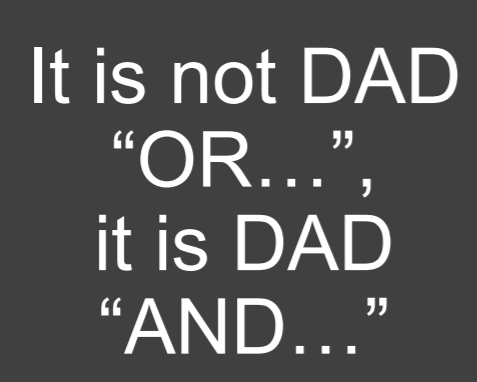
\includegraphics[scale=1]{dad-topic.png}
	\caption{Was DAD ist.}
	\label{fig:birds}
\end{figure}

